\documentclass[25pt,halfparskip-,pagesize]{scrartcl}
\usepackage[papersize={34in,44in},body={780mm,1000mm},top=.5in,ignoreheadfoot]{geometry}
\usepackage{eso-pic}
\usepackage{bera}
\usepackage{fourier}
\usepackage[scaled]{luximono}
\usepackage[T1]{fontenc}
\usepackage[english]{babel}
\usepackage{graphicx,color,multicol,booktabs,listings,fancybox,calc}
\usepackage{capt-of}
\usepackage{subfigure}
\usepackage{tabularx}
%\raggedcolumns
\flushcolumns

%\show\hrulefill
\AddToShipoutPicture{%
    \AtPageUpperLeft{\makebox(0,0)[lt]{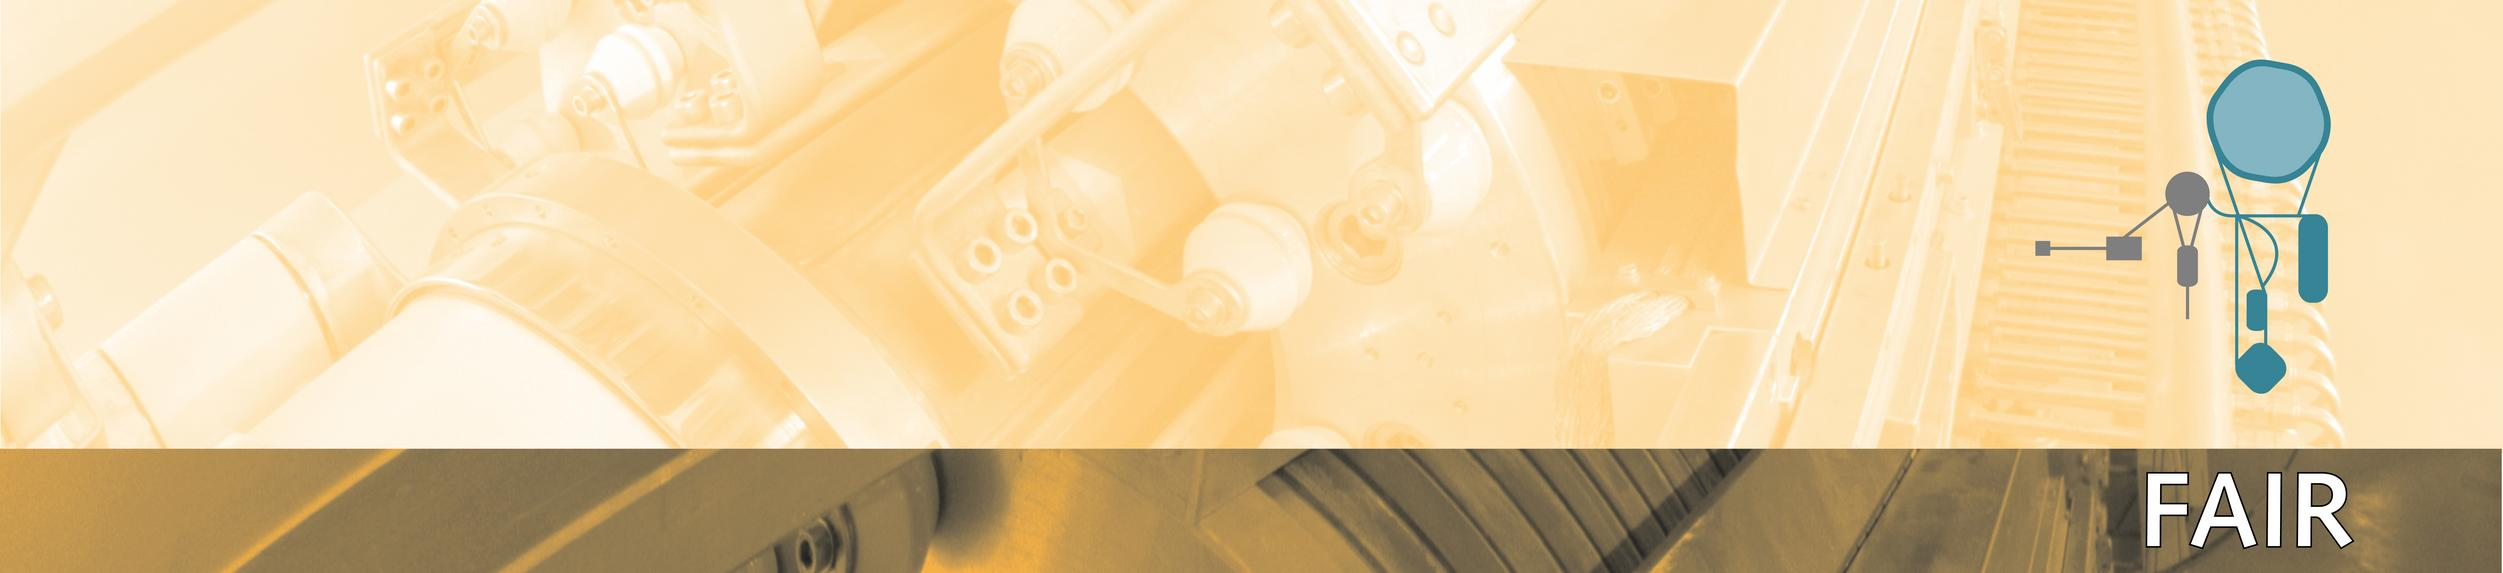
\includegraphics[width=\paperwidth]{head-small}}}
    \unitlength1cm
    \AtPageUpperLeft{\kern5cm\lower9cm\hbox{
\includegraphics[width=11cm]{../images/GSI_Logo_cmyk.eps}}}
    \AtPageUpperLeft{\kern.1cm\rule[-.3cm]{.4pt}{.2cm}}
    \AtPageUpperLeft{\kern.1cm\rule[-.1cm]{.2cm}{.4pt}}
    \AtPageUpperLeft{\kern\paperwidth\kern-.1cm\rule[-.3cm]{.4pt}{.2cm}}
    \AtPageUpperLeft{\kern\paperwidth\kern-.3cm\rule[-.1cm]{.2cm}{.4pt}}
    \AtPageLowerLeft{\kern.1cm\rule[.1cm]{.4pt}{.2cm}}
    \AtPageLowerLeft{\kern.1cm\rule[.1cm]{.2cm}{.4pt}}
    \AtPageLowerLeft{\kern\paperwidth\kern-.1cm\rule[.1cm]{.4pt}{.2cm}}
    \AtPageLowerLeft{\kern\paperwidth\kern-.3cm\rule[.1cm]{.2cm}{.4pt}}
    \linewidth2pt
    \AtPageLowerLeft{\kern1in\kern\oddsidemargin\lower-3cm\hbox to \textwidth{\leaders \hrule height \linewidth \hfill \kern 1cm\lower.5cm\hbox{
\includegraphics[height=2cm]{../images/GSI_Logo_cmyk.eps}}\kern1cm\rule{3cm}{\linewidth}}}
    \AtPageLowerLeft{\kern1in\kern\oddsidemargin\lower-2cm\hbox{\sffamily\fontsize{12pt}{12pt}\selectfont PCaPAC\,2012}}
}

\def\TTra{\textsuperscript{\texttrademark}}
\definecolor{title}{cmyk}{.00,0.15,0.75,0}
\definecolor{solution}{cmyk}{.10,1.00,.80,0}
%\definecolor{colsection}{cmyk}{1,.8,0,0}
\definecolor{colsection}{cmyk}{0,.6,.6,.7}
\definecolor{itemgreen}{cmyk}{1,0,.9,.2}
\definecolor{itemroyalblue}{cmyk}{.711,.533,0,.118}
\definecolor{itemblue}{cmyk}{1,1,0,.2}
\definecolor{lstbackground}{cmyk}{0.35,0.05,0.0,0.0}
\definecolor{lstemph}{cmyk}{0.0,1.0,0.95,0.0}
\definecolor{lstbackgroundalt}{cmyk}{0.05,0.05,0,0.2}
\definecolor{lststring}{cmyk}{.6,1,.8,0}
\newcommand{\solution}[1]{\textbf{\textcolor{solution}{#1}}}
\setkomafont{descriptionlabel}{\itshape}
\setcounter{secnumdepth}{-1}
\pagestyle{empty}
\addtokomafont{section}{\color{colsection}}
\addtokomafont{caption}{\itshape}
\setlength{\columnsep}{5em}
\newcommand\mycaption[1]{\textit{#1}}
%\renewcommand{\familydefault}{\rmdefault}

\usepackage{pifont}
\renewcommand*\labelitemi{\color{colsection}\ding{110}}
\renewcommand*\labelitemii{\color{itemgreen}\ding{108}}

\lstset{showstringspaces=false,basicstyle=\ttfamily\small,
    keywordstyle={\bfseries},stringstyle={\color{lststring}},tabsize=4,framerule=2pt,rulecolor=\color{black},
    rulesep=5pt,abovecaptionskip=6pt,belowcaptionskip=8pt,
    emphstyle=\color{lstemph}}

\lstdefinelanguage{nodal}
}

\newcommand\class[1]{\texttt{#1}}

\makeatletter
\DeclareRobustCommand{\Cpp}
{\valign{\vfil\hbox{##}\vfil\cr
   C\kern-.05em\cr
      %$\hbox{\fontsize{\sf@size}{0}+\kern-0.05em+}$\cr}%
      \hbox{+\kern-0.05em+}\cr}%
}
\makeatother

\setlength{\fboxsep}{1em}
\raggedright
\begin{document}
\vspace*{1ex}

{\centering
\begin{minipage}{20in}
\centering \sffamily\Huge \rule{0pt}{50pt}\textbf{Facility-Wide Synchronization of Standard FAIR Equipment Controllers}\par
\vspace{5mm} \LARGE Stefan Rauch,
Wesley Terpstra,
Wolfgang Panschow,
Matthias Thieme,
Cesar Prados,
Marcus Zweig,
Mathias Kreider,
Dietrich Beck,
Ralph B\"ar
\par
\vspace{5mm}
\Large GSI, D-64291 Darmstadt, Germany
\rule[-12pt]{0pt}{10pt}\par
\end{minipage}%
\par}%

%\vspace{11cm}
\vspace{6.5cm}
\setlength{\fboxrule}{1pt}
\begin{multicols*}{3}
\ovalbox{%
\begin{minipage}{\linewidth}
\section{Abstract}
\small The standard equipment controller under development for the new FAIR
accelerator facility is the Scalable Control Unit (SCU). It is designed to
synchronize and control the actions of up to 12 purpose-built slave cards,
connected in a proprietary crate by a parallel backplane. Inter-crate
coordination and facility-wide synchronization are a core FAIR requirement
and thus precise timing of SCU slave actions is of vital importance.

The SCU consists primarily of two components, an x86 COM Express daughter
board and a carrier board with an Altera Arria II GX FPGA, interconnected by
PCI Express. The x86 receives configuration and set values with which it
programs the real-time event-condition-action (ECA) unit in the FPGA. The
ECA unit receives event messages via the timing network, which also
synchronizes the clocks of all SCUs in the facility using White Rabbit.
Matching events trigger actions on the SCU slave cards such as: ramping
magnets, triggering kickers, etc.

Timing requirements differ depending on the action taken. For softer
real-time actions, an interrupt can be generated for complex processing on
the x86. Alternatively, the FPGA can directly fire a pulse out a LEMO output
or an immediate SCU bus operation. The delay and synchronization achievable
in each case differs and this paper examines the timing performance of each
to determine which approach is appropriate for the required actions.
\par
\end{minipage}}

\section{Introduction}
In the FAIR control system,
a data master issues high-level commands to control accelerator devices.
The front-end controllers in the system reacts to relevant commands,
issuing appropriate actions to their hardware components.
Depending on the action to be taken, there are different timing requirements to be met.

\begin{itemize}
  \item commands carry absolute execution timestamp
  \item time limit for frond-end controllers for receiving commands
  \item depending on the time for processing an action
  \item tradeoff between responsivness and planning ahead
\end{itemize}

Non-deterministic execution time is a potentially much more serious problem.
For example, if a kicker executes an action a few nanoseconds too late,
the beam might be lost.
However, not all actions require the same precision,
and it may make sense to trade accuracy for flexibility in some situations.
Fortunately, the  most common equipment controller in FAIR,
the Scalable Control Unit (SCU),
has several possibilities for executing actions.
This paper outlines the timing requirements of various accelerator
components in FAIR and explorers the alternatives which could meet them.

\section{Use Cases}
\begin{itemize}
	\item main frontend controller for the FAIR project
        \item different slaves for different use cases
        \begin{itemize} 
	  \item Adaptive Control Units (ACU) for power supplies
          \item FPGA Interface Board (FIB) for Radio Frequency (RF) control
          \item Kicker modules controlled by IFK via MIL-STD-1553 based field bus
        \end{itemize}
\end{itemize}

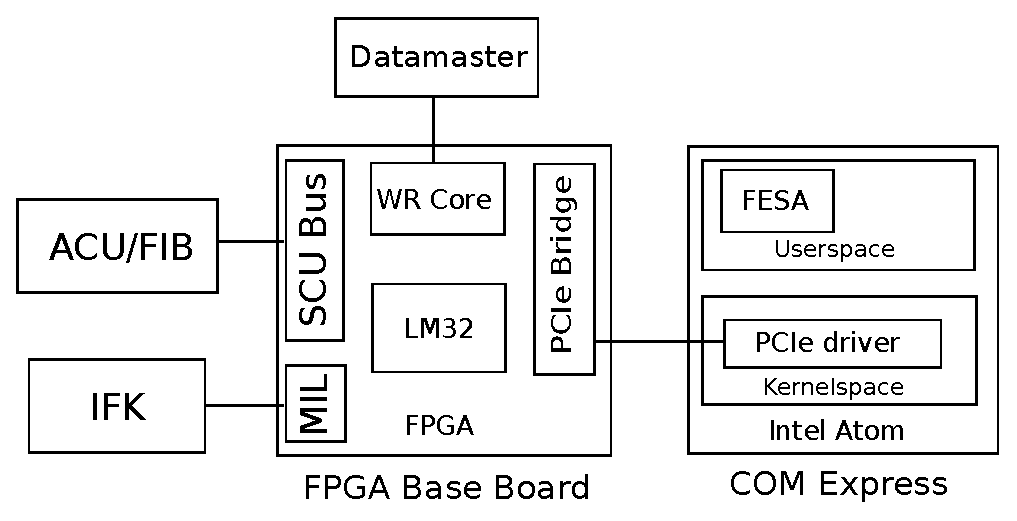
\includegraphics[width=\columnwidth]{../images/WEPD48f2}
\captionof{figure}{Block diagram of SCU}
\label{fig:block_diagram}



\section{Scalable Control Unit (SCU)}
\begin{itemize}
  \item stack of up to three separated boards
  \item base board with Arria II FPGA, 2 SFP slots, DDR3 RAM, parallel flash, SCU bus
  \item White Rabbit Timing circuitry
  \item COMExpress module with Intel Atom CPU, connected via PCIe
  \item optional extension board for MIL-STD-1553 based field bus
  \item SCU receives 1ns accurate timing information via White Rabbit link
\end{itemize}

\begin{center}
  \begin{tabular}{l|c|c|c|c}

   $\mu$s    & min   & mean  & max   & stddev \\
   \hline
    FPGA      & 0 & 0.001 & 0.001 & 0.001 \\
    LM32      & 2.863 & 2.924 & 3.217 & 0.058  \\
    Kernel    & 7.120 & 13.29 & 37.73 & 3.49   \\
    Userspace & 49.36 & 62.49 & 93.33 & 5.62   \\
    FESA      & 138.9 & 170.1 & 246.1 & 10.8 \\
   \end{tabular}
  \caption{Execution timing performance}
\label{tab:stat_table}
\end{center}

\section{Execution Alternatives}
\begin{itemize}
  \item FPGA
    \begin{itemize}
      \item can be programmed to generate output on 8ns phase aligned clock edge
      \item with fine delay card down to 1ns
      \item only source of jitter is PLL of the FPGA and inherent inaccuracy of White Rabbit
    \end{itemize}
  \item LM32
    \begin{itemize}
      \item FPGA triggers soft-CPU via interrupt
      \item software generates appropriate action
      \item delay from switch time to interrupt context and running the software
      \item jitter from cache behaviour and on-chip bus access
    \end{itemize}
  \item Atom-Kernel
    \begin{itemize}
      \item FPGA interrupt directly handled in kernel
      \item delays equal to LM32 + PCIe bridge delay
      \item more jitter caused by Linux kernel
    \end{itemize}
  \item Atom-Userspace
    \begin{itemize}
      \item FPGA interrupt delivered to userspace
      \item adds delay by context switch 
    \end{itemize}
  \item FESA
    \begin{itemize}
      \item interrupt is translated to an action using threads
      \item this increases number of context switches
    \end{itemize}
\end{itemize}

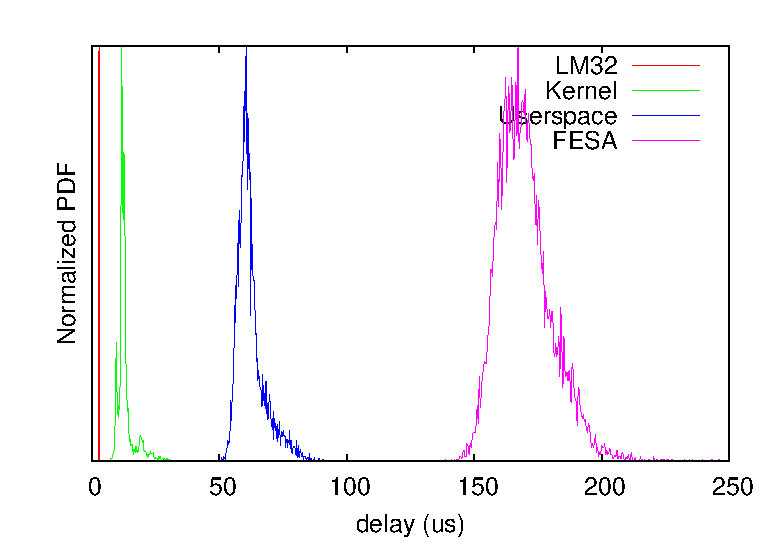
\includegraphics[width=\columnwidth]{../images/WEPD48f1}
\captionof{figure}{Comparison of delay distributions}
\label{fig:delaycomparison}

\columnbreak

\section{Analysis}
The outputs of an SCU were connected to an oscilloscope.
First output is the action aligned to FPGA's 8ns clock.
Second output is toggled by execution path. The approach
ignores FPGA execution time.
All test were done with background load and with at least
10000 samples. Load for LM32 was White Rabbit PTP core and
save/restore of all 32 registers on interrupt context switch.
The Atom was streaming text over ssh.
Test were done with real-time patched 2.6.33.6 Linux kernel.
The PCIe bridge interrupt handler and tasklet process were
set to priority 99, the userspace test program to 98. FESA
set its own priority to 60.
We also measured the LM32 without instruction cache. This reduced
the variability from 354ns to 272ns. Average delay was increased
from 2.924$\mu$s to 3.810$\mu$s. Most of the variability seems
to stem from Wishbone operations.
The LM32 was clocked at 62.5Mhz and when zoomed into the plot
around 3$\mu$s you can see a distribution of 22 spikes with 16ns
intervals (Figure ~\ref{fig:lm32plot}).
The time from interrupt to the handler in Linux and the time
from interrupt handler to userspace varies significantly.
With 10000 samples the worst case delay was 240$\mu$s for FESA.

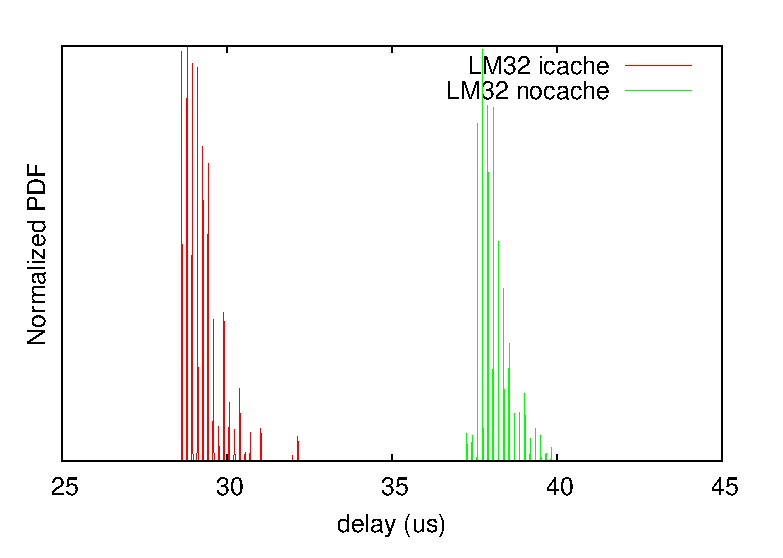
\includegraphics[width=\columnwidth]{../images/lm32plot}
\captionof{figure}{LM32 delay distribution}
\label{fig:lm32plot}

\section{Conclusion}
The measured times as presented in Figure ~\ref{tab:stat_table}
must be reviewed in the context of different use-cases. As an example,
ramping of magnets must be done synchronously. Here, a guaranteed
synchronicity of 10-20$\mu$s must be achieved for ring machines like the
SIS18 and the SIS100. Another example is the control of kicker magnets,
which requires  at least 3ns precision and can only be done with FPGA
Hardware Description Language (HDL). Software on the COM Express module
may only be used for cases, where hard real-time is not required.
None of the solutions involving the CPU on the COM Express module fulfill
those requirements, as long as the use of real-time Linux as operating
systems is a stringent requirement for software tools like FESA.

For hard real-time the options are FPGA HDL or LM32 software. Here, FPGA
HDL provides nanoseconds timing while LM32 software provides a better
flexibility. To avoid stringent limitations for future developments of
the FAIR accelerator complex, standard FAIR equipment controllers like
the SCU should be designed to support hard real-time on the nanoseconds
scale. If flexibility during runtime is required, the ideal solution
could be a combination of both options, where LM32 software creates the
action patterns that are phase aligned with high precision by FPGA HDL.


\vfill

\end{multicols*}
\end{document}
